\documentclass[a4paper,12pt]{article}

\RequirePackage{epsfig}

\setlength\hoffset{-0.5in}      %% these work quite well with a 12pt font
\setlength\voffset{-0.5in}
\setlength{\textwidth}{6.30in}
\setlength{\textheight}{9.0in}

\usepackage{longtable}
\usepackage{array}
\usepackage{graphicx}
\usepackage{float}
\usepackage{enumitem}
\usepackage{hyperref}
\graphicspath{ {./img/} }

\bibliographystyle{unsrt}
\begin{document}

\begin{center}
{\Large\bf{Decentralised Blockchain Security Architecture for IoT and MQTT Brokers}} \\
      \vspace{5.0mm}
{\Large\bf{Project Plan}} \\
      \vspace{8mm}
      {\large\bf{Konrad Dryja}}  \\
      \vspace{5.0mm}
       {\tt k.dryja.15@abdn.ac.uk} \\
      \vspace{5.0mm}
      {\em Department of Computing Science,\\
       University of Aberdeen, Aberdeen AB24 3UE, UK} 
\end{center}


\section*{Introduction}

Internet of Things (further referred as IoT) is a growing field with its presence getting larger from day to day. Equipment such as bus timetables, doorbells, thermostats or even pacemakers capable of sending alerts directly to emergency services are omnipresent. It's a system of computers, chips, phones, sensors deployed in our lives capable of communicating with each other without requiring any human intervention.

Sensitive data is very often handled and leak or misrepresentation can have catastrophic consequences. Additionally, those devices have limited computation power, which is sacrificed in favour of extended lifespan to avoid frequent maintenance and/or battery replacement. This makes it a very lucrative target for malicious actors. Researchers from University of Michigan performed a demo attack on a pacemaker, extracting personal information and changing the configuration.\cite{4531149} This example and more clearly presents a need for solution capable of securing and closing off access to unwanted agents.

What is more, those devices frequently do not directly communicate on a peer-to-peer basis, but instead pass through intermediary resource handling the distribution of data. MQTT Brokers\footnote{\url{https://mqtt.org/}} are one of them, providing a Publisher/Subscriber architecture, allowing for information exchange without the constant need of interconnectivity between clients, instead of relying on created topics used as a relay. It's very important to point out that MQTT is not a piece of software, but rather a standard describing the operation of such backend and leaves the implementation up to end-users - the implementation is very often referred as MQTT brokers.

The documentation also clearly states that the security is not a part of the standard, but rather leaves this decision up to the implementors, offering several alternatives\footnote{\url{https://docs.oasis-open.org/mqtt/mqtt/v5.0/os/mqtt-v5.0-os.html\#\_Toc3901261}}. And while the transport of data can be assumed to remain secure (as MQTT operates over TCP/IP, thus encrypting the data using TLS), the access is often not. For example, an attack could be conducted, where malicious device communicates with the broker, impersonating another IoT hardware and finally compromise confidentiality.

\begin{figure}[ht]
  \centering
  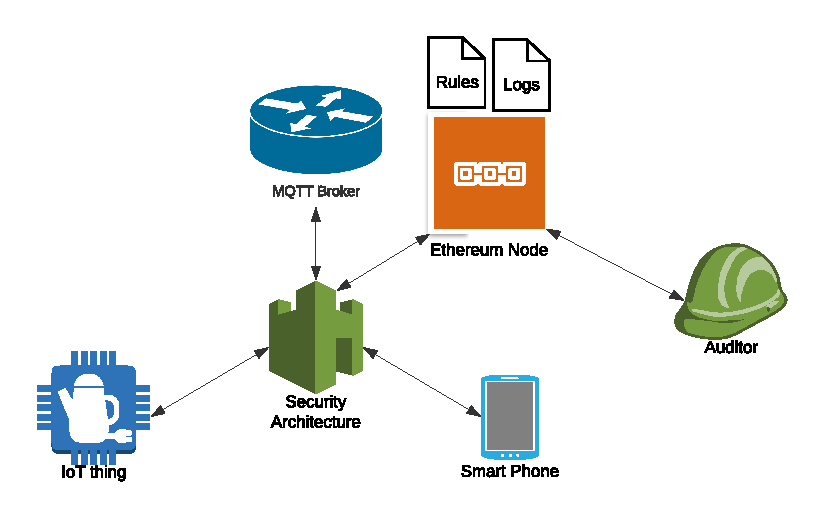
\includegraphics[scale=0.8]{iot_attack}
  \caption{Proposed architecture}\label{fig:iot1}
\end{figure}

Common implementation of MQTT brokers includes basic authentication based on a username and a secret password, offering limited to no logging capabilities. For example, one of the most popular brokers being Mosquitto\footnote{\url{https://mosquitto.org/man/mosquitto-conf-5.html}}, as of version 1.6.8 offers password based authentication with ACL capabilities restricting some credentials only to given topics. Related effort was presented in TrustLens project from University of Aberdeen presenting solution of attaching semantic annotations to ongoing operation of a broker and in process allowing higher transparency of broker's state\cite{10.1145/3366610.3368099}. And while it does not provide neither Authentication nor Authorization, it tackles Accountability.

I would like to propose a universal, pluggable module following the description of MQTT standard (and thus potentially making it independent from the used MQTT Broker) handling Authentication, Authorization and Accountability of IoT devices and consumers attempting connection to the brokers. In order to make the platform more resilient and independent from single points of failure (often being the central ACL repository), I will deploy it on a blockchain - which by convention supports recording of transactions (by placing them on the blockchain) and authentication via ID of the presented wallet. Figure \ref{fig:iot1} represents sketch of the proposed architecture, where the Security element would handle all incoming connections and proxy them accordingly. Due to the public nature of blockchain architecture, transactions would also be available to view by third parties for the purposes of auditing and transparency.

As mentioned, logging (that is, Accountability) will be the main focus of the project. Normally, it would not be feasible to record every event happening on the broker, as the number operation would greatly exceed the storage capacity. Relevant rules that would determine whether the event is worth recording or not would be created, those could include multiple failed attempts, high-profile operations (handling PII) or administrative tasks (such as permission changes).

Preliminary research revealed similar efforts by scientist in Khon Kaen University~\cite{8523942}, although focusing mostly on Hyperledger Fabric and optimization of the configuration through Genetic Algorithms. The paper doesn't make any mention of logging and provenance functionality, which I would like to put more attention towards - along with focusing on Ethereum platform instead.


\section*{Goals}

The project can be divided onto main goals and extras, leaving some field for maneuvering in case of road blocks or difficulties resulting from the challenges faced in the dissertation. By having flexible targets, I will be able to stop sooner in case of overestimating the schedule, or carrying on with extra work, should I find myself meeting the targets quicker than expected. Moreover, I would like to also put some attention to listing the things that the project is \textbf{not} trying to be, to avoid sidetracking.

\paragraph{Main Goals:}
\begin{itemize}
  \item Design Blockchain network, relevant data models that would be placed on the blockchain and deploy on Ethereum platform, capable of recording transactions and allowing for modification of ACLs, i.e. which wallet ID is permitted to access given topics. Part of this goal would also be determining which information is important enough to be recorded and which should be discarded.
  \item Design rules and data models that would drive the premise behind the rules used for data capture. 
  \item Design containerised software acting as a secure proxy between brokers and connecting clients. This will handle both authentication and logging performed action as immutable transactions. Logging would only be performed if the requested operation triggers some pre-defined rules.
  \item Deploy and test on at least one MQTT Broker (e.g. Moquette, Mosquitto), simulated with software.
\end{itemize}

\paragraph{Extra Goals:}
\begin{itemize}
  \item Create public API for the auditors to freely view the contents of blockchain and thus transactions containing information about suspicious operations.
  \item Explore and implement implementation of the architecture to any, arbitrary broker.
  \item Connect physical LoRaWAN gateways to the software.
\end{itemize}

\paragraph{No-goals:}
\begin{itemize}
  \item Design a new blockchain platform from scratch.
  \item Write / modify operating system of IoT devices.
  \item Design a new MQTT Broker -- although modification of existing solutions might be required.
  \item Create a solution for hardware identification.
\end{itemize}


\section*{Methodology}

For the project, I will be following iterative approach of fulfilling my targets, reflecting back on the sprints, which would be independent from each other (although one might rely on completion of another). Doing so would allow me to modify the requirements in case of facing blocks or difficulties that would not be feasible to solve in the given time span.

One could distinguish the following main tasks, that would be crucial when it comes to determining the success of the project:
\begin{itemize}
  \item Preliminary research revealed some related work which I will need to review (along with others) to determine main focus points on the project and to apply to findings determined in other academic papers.
  \item At the start of this project, my knowledge of blockchain networks and their implementation is very limited, a further reading and study would be required.
  \item I have also never interacted with any MQTT brokers, so familiarisation by setting up lab environment would be necessary. Either Moquette or Mosquitto would be used, depending on the findings from the literature review. The respective documentation would also be reviewed.
  \item Having reviewed background information, I can proceed to designing the architecture of my system. This can be divided onto two smaller sub-tasks:
    \begin{itemize}
      \item Design mock-ups of the system and seek peer-review on the implementation.
      \item Majority of the project involves creation of relevant rules for transactions capture.
      \item Implement the mock-ups in Golang, which would be deployed in containerised environment.
    \end{itemize}
  \item With finalised software, testing and debugging can be commenced, again can be split onto two phases.
    \begin{itemize}
      \item Testing in virtualised, hermetic environment
      \item Field tests on physical hardware. This is optional and depends on the velocity of the project.
    \end{itemize}
\end{itemize}

\section*{Resources Required}

For the purposes of the project, laptop and a workstation should be sufficient, as the MQTT brokers can be simulated via software, without the need of physical IoT devices sending the messages. For the second stage of the project, I will be considering putting the software on a physical LoRaWAN gateway, enhancing the current broker implementation. TrustLens team from University of Aberdeen recently acquired such gateway, which I will be able to use given the need. Moreover, the team also owns several PuckJS sensors and Arduino boards, which would allow to deploy the whole system and test its behaviour in the real world.

To summarize the requirements:
\begin{itemize}
  \item Linux PC with the following software: 
    \begin{itemize}
      \item Golang 1.12+ -- runtime for the server application
      \item Docker 19.03.5+ -- deployment environment
      \item Bazel 2.0.0+ -- for building the source code
      \item MQTT Broker -- this could be either Moquette or Mosquitto
      \item Suitable text editor (Vim)
    \end{itemize}
  \item Additionally, for tests in the field:
    \begin{itemize}
      \item LoRaWAN Gateway
      \item IoT sensors (PuckJS, Arduino) 
      \item Mobile Device
      \item Should the above not be sufficient, a Raspberry Pi running standard Linux environment
    \end{itemize}
\end{itemize}

Extra requirements might arise throughout the project, although I do not expect anything that might require big time or financial investments.

\section*{Evaluation}
To determine the success of the project, a substantial amount of the time will need to be spent on evaluating the performance and functionality. As my project is likely to introduce operational and performance overhead, comparison between vanilla or similar solution will have to be in order to determine the feasibility of the proposed system. Several test scenarios will be considered:
\begin{itemize}
  \item Time to process messages of new system with increasing number of messages, 100, 10k, 100k and so on.
  \item Determine whether my system is capable of stopping and/or capturing attacks which would've gone unnoticed in a vanilla MQTT Broker. This could included DoS type of attacks, brute forcing or unusual patterns of operation.
\end{itemize}

\section*{Risk Assessment}

\bgroup
\def\arraystretch{2}
\begin{table}[H]
\centering
\begin{tabular}{|m{0.4\textwidth}|m{0.4\textwidth}|m{0.1\textwidth}|}
\hline
\textbf{Risk} & \textbf{Mitigation}                       & \textbf{Level} \\ \hline
\begin{itemize}[leftmargin=*]
  \item LoRaWAN gateway owned by the university utilises a completely different tech stack, than the one that I will be working on.
  \item IoT devices run proprietary software and replacing it would require substantial amount of time.
\end{itemize} &
\begin{itemize}[leftmargin=*]
  \item Virtualise the environment, without having to physically put software on any hardware.
  \item Simple container with minimal Linux Image should be representative enough.
  \item Alternatively, purchase a new Raspberry Pi.
\end{itemize} &
Medium \\ \hline
\begin{itemize}[leftmargin=*]
  \item Ethereum doesn't meet my needs or understanding it takes substantial amount of time.
  \item I face a block relating to knowledge of Ehtereum effectively stopping me from reaching my goals.
\end{itemize} &
\begin{itemize}[leftmargin=*]
  \item Switch to an implementation that I am more familiar with, although with slightly different tradebacks, that is, Hyperledger Fabric.
\end{itemize} &
Medium \\ \hline
\begin{itemize}[leftmargin=*]
  \item Unexpected hardware failure or theft.
  \item Any hazards resulting from the natural wear and tear of utilized hardware
\end{itemize} &
\begin{itemize}[leftmargin=*]
  \item All code, documentation and report should be frequently backed up and versioned using git (and thus, uploaded to GitHub), allowing for data recovery in case of a disaster.
  \item If LoRaWAN gateway or other IoT equipment was to become faulty or technologically infeasible, focus on virtualised solutions, as per first row.
\end{itemize} &
Low \\ \hline
\end{tabular}
\end{table}
\egroup
\pagebreak
\section*{Timetable\footnote{Live version can be seen at \url{https://bit.ly/2RTiRxV}}}

\begin{figure}[ht]
  \centering
  \makebox[\textwidth][c]{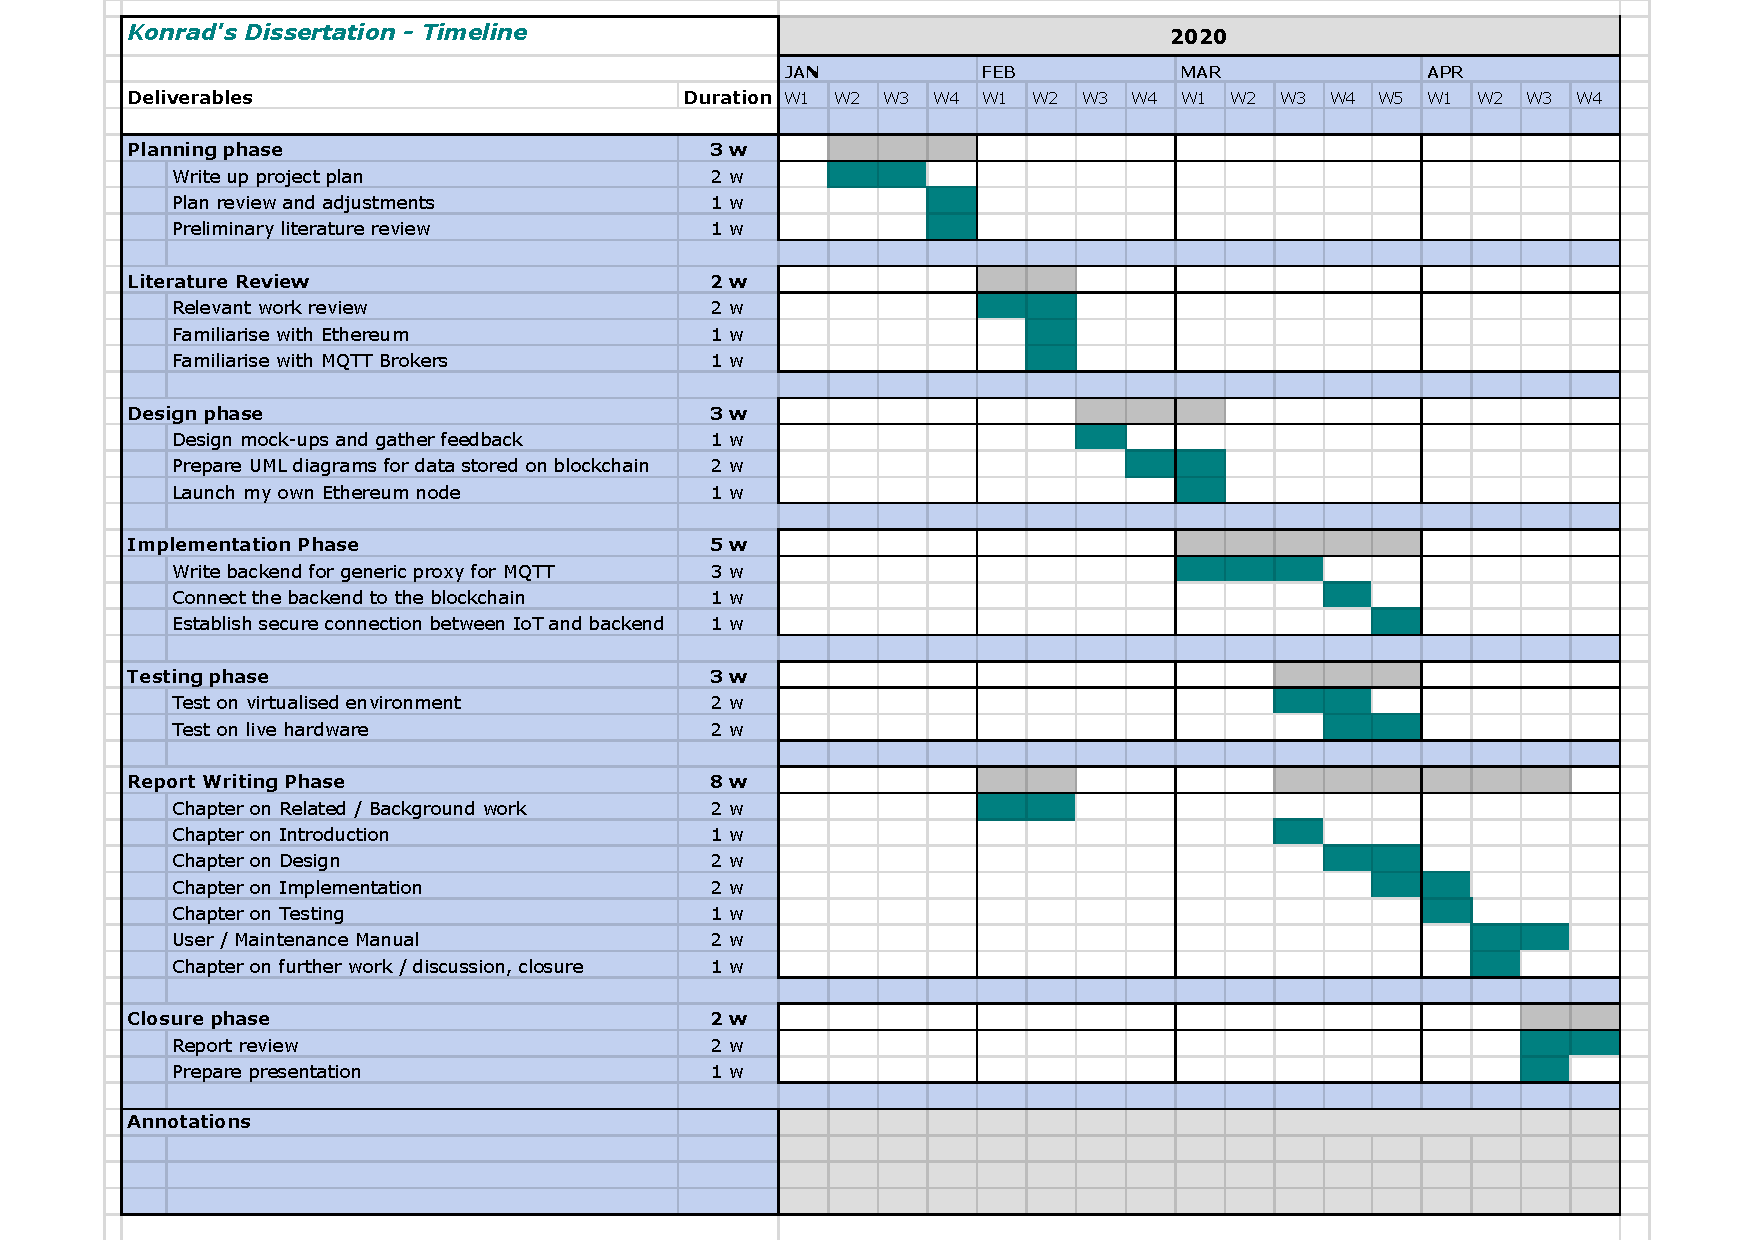
\includegraphics[scale=0.7]{timeline}}
\end{figure}

\bibliography{ProjectPlan}

\end{document}
